\documentclass[12pt, twoside]{book}
\usepackage[top=1in, bottom=1in, left=1.2in, right=1in, a4paper]{geometry}
\title{Automated Retrieval of Semantic Web Services}
\author{Adarsh Mohata, Ajith P S, Ashish Kedia}

 \ifx\pdftexversion\undefined
 \usepackage[dvips]{graphicx}
 \else
 
 \usepackage[pdftex]{graphicx}
 \DeclareGraphicsRule{*}{mps}{*}{}
 \fi
\usepackage{url}
\usepackage{tabularx}
\usepackage{chapterbib}
\usepackage{hyperref}
\usepackage{lscape}
\usepackage{longtable}
\usepackage{float}
\usepackage{url}
\usepackage{amsmath}
\usepackage{multicol}
\usepackage{color}
\usepackage[utf8]{inputenc}
\usepackage{listings}
\usepackage{kbordermatrix}
\usepackage{fancyhdr}
\usepackage{caption}
\usepackage{chngcntr}
\usepackage{pdfpages}
\usepackage{amsmath}
\counterwithin{figure}{chapter}
\counterwithin{table}{chapter}
%\pagestyle{fancy}
\lhead{\leftmark}
\rhead{}
\cfoot{}
\rfoot{\thepage}
\raggedbottom
\renewcommand{\bibname}{References}
\newcommand{\project}{Automated Retrieval of Semantic Web Services}
\setcounter{secnumdepth}{4}
\setcounter{tocdepth}{4}

\definecolor{codegreen}{rgb}{0,0.6,0}
\definecolor{codegray}{rgb}{0.5,0.5,0.5}
\definecolor{codepurple}{rgb}{0.58,0,0.82}
\definecolor{backcolour}{rgb}{0.95,0.95,0.92}

\lstdefinestyle{mystyle}
{   language=bash,
    basicstyle=\ttfamily,
    morekeywords={peter@kbpet},
    alsoletter={:~\$},
    morekeywords=[2]{peter@kbpet:},
    keywordstyle=[2]{\color{red}},
    literate={\$}{{\textcolor{red}{\$}}}1 
	    {:}{{\textcolor{red}{:}}}1
	    {~}{{\textcolor{red}{\textasciitilde}}}1,
    backgroundcolor=\color{backcolour},	  
    commentstyle=\color{red},
    keywordstyle=\color{blue},
    numberstyle=\tiny\color{codegray},
    stringstyle=\color{codepurple},
    basicstyle=\footnotesize,
    breakatwhitespace=true,         
    breaklines=true,                 
    captionpos=b,                    
    keepspaces=true,                 
    numbers=left,                    
    numbersep=5pt,                  
    showspaces=false,                
    showstringspaces=false,
    showtabs=false,                  
    tabsize=4
}

\begin{document}
\begin{titlepage}
 \begin{center}
	\emph{A Mini-Project Report on} \\
\vspace{1cm}
\large
\textbf{Automated Retrieval of Semantic Web Services} \\
\normalsize
\vspace{1cm}
\emph{carried out as part of the course Web Technologies and Applications $(IT$ $302)$} \\
\vspace{1cm}
\emph{Submitted by} \\
\vspace{1cm}
\textbf{Adarsh Mohata - 12IT03 - $V$ Sem B.Tech} \\
\vspace{4mm}
\textbf{Ajith P S - 12IT04 - $V$ Sem B.Tech} \\
\vspace{4mm}
\textbf{Ashish Kedia - 12IT14 - $V$ Sem B.Tech} \\
\vspace{1cm}
\emph{in partial fulfillment for the award of the degree} \\
\vspace{7mm}
\emph{of} \\
\vspace{7mm}
\textbf{Bachelor of Technology} \\
\vspace{7mm}
\emph{in} \\
\vspace{7mm}
\textbf{Information Technology}
\vspace{1cm}
\begin{figure}[H]
	\centering
	
\includegraphics[height=3.5cm]{pics/nitk_logo.jpg}
\end{figure}
\vspace{1cm}
\textbf{Department of Information Technology} \\
\vspace{5mm}
\textbf{National Institute of Technology Karnataka Surathkal} \\
\vspace{5mm}
\text{November 2014}
\end{center}
\end{titlepage}

 \pagebreak \textcolor{white}{text}
\thispagestyle{empty}
\pagenumbering{gobble}
\pagebreak
\begin{center}
\Huge
\textbf{Web Technology Mini Project} \\
\textbf{Project Approval Certificate} \\
\vspace{1cm} \Large
\textbf{Department of Information Technology} \\ \vspace{0.5cm}
\textbf{National Institute of Technology Karnataka Surathkal}
\vspace{3cm}
\end{center}
This is to certify that the project entitled \textbf{\project} is a bona-fide work carried out as part of the course Web Technologies and Applications (IT 302), under my guidance by \textbf{Adarsh Mohata}, \textbf{Ajith P S} and \textbf{Ashish Kedia} of $V^{th}$ Sem B.Tech (IT) at the Department of Information Technology, National Institute of Technology Karnataka, Surathkal, during the fifth academic semester in partial fulfillment of the requirements for the award of the degree of Bachelor of Technology in Information Technology, at NITK Surathkal.  \\
\vspace{3cm}
\\
\begin{tabular}{l@{\hskip 4cm} r}
	\line(1,0){150} & \line(1,0){150} \\
	 Gaurav Prasad &  Shridhar Sanshi \\
	 Dept. of IT, NITK & Dept. of IT, NITK \\
	 Project Mentor & Project Mentor \\ 
\end{tabular}

\vspace{4cm}
\begin{flushleft}
Place: NITK Surathkal, Mangalore \\
Date: \today
\end{flushleft}
\pagebreak \textcolor{white}{text} \pagebreak
\thispagestyle{empty}
\begin{center}
\Huge
\textbf{Declaration} \\
\end{center}
We hereby declare that the project entitled \textbf{\project} submitted as part of the partial course requirements for the course \textbf{Web Technologies and Applications (IT 302)} for the award of the degree of Bachelor of Technology in Information Technology at National Institute of Technology Karnataka, Surathkal during the fifth academic semester (July, 2014 - November, 2014) has been carried out by us and where others' ideas or words have been included, we have adequately cited and referenced the original sources. We declare that the project has not formed the basis for the award of any degree, associateship, fellowship or any other similar titles elsewhere. \\
Further, We declare that we will not share, re-submit or publish the code, idea, framework and/or any publication that may arise out of this work for academic or profit purposes without obtaining the prior written consent of the course Faculty Mentor and Course Instructor \\
\vspace{2cm}

\begin{tabular}{@{\hskip 5.3cm}r}
	\line(1,0){150} \\
	Mr. Adarsh Mohata \\
	Department of Information Technology \\
    National Institute of Technology Karnataka, Surathkal\\
    \vspace{1cm} \\
    
    \line(1,0){150} \\
	Mr. Ajith P S \\
	Department of Information Technology \\
    National Institute of Technology Karnataka, Surathkal\\
    \vspace{1cm} \\
    
    \line(1,0){150} \\
	Mr. Ashish Kedia \\
	Department of Information Technology \\
    National Institute of Technology Karnataka, Surathkal\\
\end{tabular}

\vspace{2cm}

Date: \underline{\hspace{5cm}}

\pagebreak \textcolor{white}{text} \pagebreak
\thispagestyle{empty}
\begin{center}
\Huge
\textbf{Acknowledgements} \\
\vspace{2cm}
\end{center}
We have put our best efforts in this project.
However, it would not have been possible without the kind support and help of many individuals.
We would like to extend our sincere thanks to all of them.\\ \par
We are highly indebted to \textbf{Mr. Shridhar Sanshi} and \textbf{Mr. Gaurav Prasad} for their guidance and constant supervision as well as for providing necessary information regarding the project and also for their support in completing the project.\\ \par
We would specially like to thank \textbf{Mrs Sowmya Kamath} for providing us with sample data-set to carry out our experiments.\\ \par
We would like to express our gratitude towards the members of Department of Information Technology for their kind co-operation and encouragement which helped us in the completion of this project. Our thanks and appreciations also go to our colleagues in other groups in developing the project and people who have willingly helped us out with their abilities.

\pagebreak \textcolor{white}{text} \pagebreak
\thispagestyle{empty}
\begin{center}
	\textbf{ \huge Abstract}
\end{center}
\vspace{1cm}
As Web services increasingly become important in distributed computing, some of the flaws and limitations of this technology become more and more obvious. One of this flaws is the discovery of Web services through common methods. Research has been pursued in the field of ”Semantic Web services”. This research is driven by the idea, to describe the functionality of Web services as accurately as possible and to create programs automatically out of already existing Web services. \\ \par
Consideration of the web service interfaces(input/output) is also equally important. It is possible to index web services available on web and find other web services with similar interfaces.\\
\par
This project aims at exploring the various ways of discovering, indexing and searching semantic web services based on their corresponding description documents. \\
\par
\textbf{Keywords : }Web Service Discovery, WSDL, OWL-S, Co-Sine Similarity

\thispagestyle{empty}
\listoffigures
\listoftables
\tableofcontents

\setcounter{page}{1}
\pagenumbering{arabic}

\chapter{Introduction}
A web service is a software system identified by a URI whose public interfaces are defined and described using XML. It interacts with other systems in a manner prescribed by it's definition thereby satisfying one or more needs of the other system. \\ \par
Web Service technologies have advanced the development of Internet-based applications by facilitating the integration and interoperability of services provided by different organizations. As a result, instead of developing monolithic applications, today, we build large-scale software applications by composing loosely coupled services. By doing so, we can reuse and select suitable services as various organizations can provide similar services for the development of different applications \cite{context_aware}.
\begin{figure}[H]
	\centering
	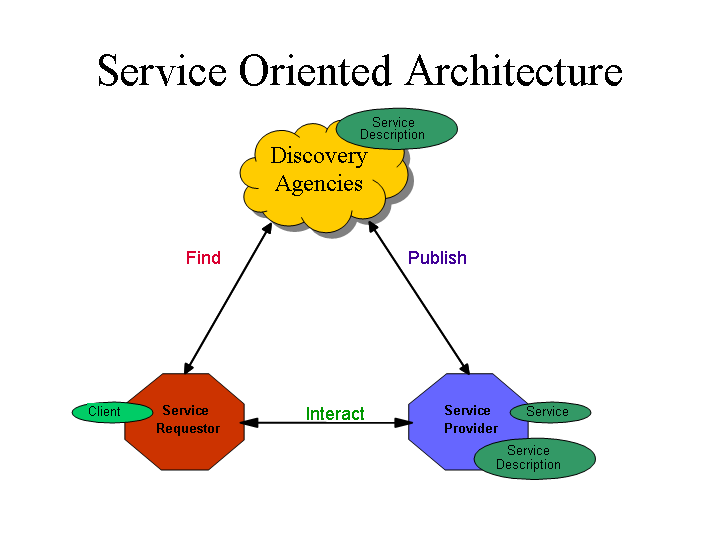
\includegraphics[width=\textwidth]{pics/soa.png}
	\caption{\textbf{Service Oriented Architecture \cite{web_arch_website}}}
\end{figure}

\section{Web Service Discovery}
When services are loosely coupled to provide functions for a particular application, it is not easy to search for the best available for a given task/application. Web Service Discovery and Retrieval often becomes a bottleneck. \\ \par
Searching proper web services is the basic step to composite web services into applications. The requirement of automated web service discovery arises in many Service Oriented Computing applications. Recent years have seen a tremendous growth in number of web services over Internet and the various standards in which the services are being described which make automated service discovery challenging and cumbersome task. \\ \par
\begin{figure}[H]
 \centering
 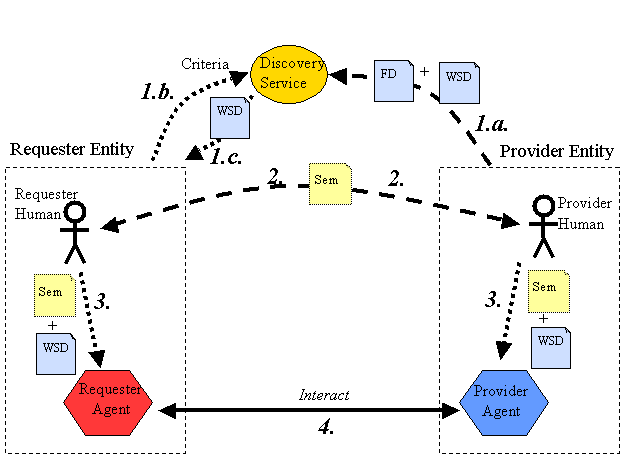
\includegraphics[width=\textwidth]{pics/discovery_process.png}
 \caption{\textbf{Web Service Discovery Process}}
\end{figure}


\section{Semantic Web Services}
Semantic Web technology is a promising first step for automated service discovery. Most current approaches for web service discovery cater to semantic web services, i.e., web services that have semantic tagged descriptions. It is difficult, however, to expect all new services to have semantic descriptions associated. Furthermore, the descriptions of the vast majority of already existing services do not have explicitly associated semantics. There are also severe restrictions on the prospective conversion of existing, non-semantic, descriptions, e.g., Web Service Description Language (WSDL), to corresponding semantic descriptions, e.g., OWL-based Web Service Ontology (OWL-S). \\ \par

\section{Purpose of the Project}
The purpose of this project is to study the existing methods of discovering web services and implement a prototype semantic web service search engine which should index a set of web services using their descriptive documents and discover appropriate services based on user's need. \\ \par
The purpose of this document is to give an overview about the work done and challenges faced by us during the course of this project.

\section{Abbreviations and Definitions}
Table ~\ref{tab: abbv} lists all the common abbreviations used throughout the length of this document and their corresponding definition.
\begin{table}[h]
	\begin{center}
		\caption{\textbf{List of Abbreviations}}
		\begin{tabular}{| p{0.2\textwidth} | p{0.6\textwidth} |}
			\hline
			\multicolumn{1}{|c|}{} & \multicolumn{1}{c|}{} \\
			\multicolumn{1}{|c|}{\textbf{Abbv}} & \multicolumn{1}{c|}{\textbf{Definition}} \\
			\multicolumn{1}{|c|}{} & \multicolumn{1}{c|}{} \\
			\hline
			PHP & PHP: Hypertext PreProcessor \\ \hline
			HTML & Hyper Text Markup Language \\ \hline
			JS & JavaScript \\ \hline
			WSDL & Web Service Description Language \\ \hline
			OWLS & Ontology Web Language Services \\ \hline
			URI & Uniform Resource Identifier \\ \hline
			UDDI & Universal Description, Discovery and Integration \\ \hline
			RDF & Resource Description Framework \\ \hline
		\end{tabular}
	\end{center}
	\label{tab: abbv}
\end{table}

\section{Outcome of Literature Survey}
After gaining an insight about the popular existing techniques used to discover web services we came to the following conclusions :
\begin{itemize}
 \item Public repositories of UDDI registries are now obsolete. Modern web services are described using ontology based OWLS and RDF.
 \item Using techniques like Natural Language Processing was out of the project's scope given the time constraint
 \item We decided to build a prototype system using conceptual indexation of service interfaces
 \item We also had an intuition that vector space search along with cosine similarity would yield a better result
\end{itemize}

\section{Problem Statement}
Retrieve description documents of various web services - WSDL and OWLS, available on the Internet and then index them efficiently so as to discover appropriate web services based on the desired service interface specified by the user's query. The system should provide users with a feature that can tune or shortlist the results.

\section{Objectives}
A major part of this work is to come up with techniques that can enhance the existing web service discovery and retrieval methods. The objectives of the project are as follows :
\begin{itemize}
 \item Retrieve XML ( WSDL and OWL-S ) documents that describes the web services
 \item Selection of Service Categories or Vector Fields
 \item Adding keywords related to each category / vector field
 \item Extracting interfaces of Web Services using their descriptive documents
 \item Indexing the retrieved web services and it's interfaces conceptually
 \item Retrieving user's required interfaces and search parameters
 \item Finding similar web services and returning the results to users
\end{itemize}
We have focused on discovering an appropriate semantic web service(s) for a given application, given the required interfaces i.e., input and output format. \\

\chapter{Methodology}
This chapter describes the methodology used for achieving the desired objectives of the project. The following sections gives a brief overview of the techniques and algorithms used as a part of our project.

\section{Retrieving Web Service Description Files}
Any system which is based on indexing of files needs a data set. In our system the data set consist of valid WSDL and OWLS files. Initially we tried retrieving the WSDL files through a Web Crawler but it was very time consuming and the resulting number of WSDL file were not so impressive. We then searched for UDDI registries which would contain lots of WSDL files. Since all the major UDDI registries were down we could only find three registries which were still functional. We successfully retrieved 470 WSDL files. All the WSDL files were downloaded using Cross Domain Scripts. Many difficulties were faced during this period, the details of which can be found in the implementation section. Unfortunately, WSDL files are obsolete and are rarely used nowadays. The new method of describing Web Services is through OWLS files. We obtained an OWLS data set through our Project Mentor.

\section{Indexing Web Service Description Files}
Each and every Web Service has, in their profile part, a set of elements named \textbf{$<<$profile:hasinput$>>$} and \textbf{$<<$profile:hasoutput$>>$}. These elements specify the respective interface of the corresponding web service. We use these interfaces to index the web services conceptually. A sample OWLS file defining the interfaces of it's corresponding web services has been shown in figure ~\ref{fig: owl}
\begin{figure}
 \centering
 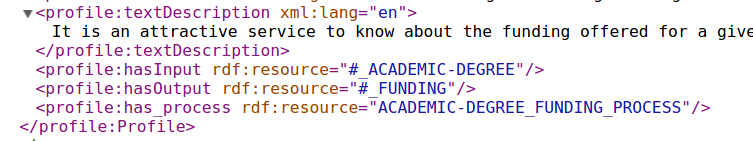
\includegraphics[width=\textwidth]{pics/sample_owls.png}
 \caption{\textbf{A sample OWLS file showing interface of the service}}
 \label{fig: owl}
\end{figure}
\par
In general any OWLS documents in our dataset can be segmented into one or more of the following classes:
\begin{enumerate}
 \item Economy
 \item Communication
 \item Education
 \item Food
 \item Weapon
 \item Medical
 \item Travel
\end{enumerate}

To index a single OWLS document, we created a OWLS Document Parser. It parses the OWLS document and extracts the required elements i.e \textbf{$<<$profile:hasinput$>>$} and \textbf{$<<$profile:hasoutput$>>$}. \\ \par
We create 2 vectors namely $V_{i}$ and $V_{o}$. Vector $V_{i}$ contains the inputs and the concepts which sum them up in the ontology (each concept will have a number which represents its frequency of occurrence in the \textbf{$<<$profile:hasinput$>>$} element of the OWLS document to which it belongs). \\ \par
We apply the same procedure to the \textbf{$<<$profile:hasoutput$>>$} element of the OWLS document and obtain the vector $V_{o}$. Thus we obtain a pair of vectors which represents an OWLS document in a vector space of 7 dimensions where each dimension is a concept. We repeated this procedure for each and every OWLS file in our data set and the resulting data contains vector representation of every OWLS document that we have in our data set. This concludes the indexing of OWLS documents and thus the corresponding web service.

\section{Searching Web Services}
We intended to create a framework through which a user could retrieve an OWLS document based on his/her needs as provided through his/her inputs. This input is nothing but the interface of the web service. For that we needed to have the capability of searching our data set, given the user's query. Our system takes the user's input and index it to obtain two vectors $S_{i}$ and $S_{o}$ similar to the procedure mentioned previously in the case of indexation of OWLS documents. \\ \par
After obtaining the two vectors we used the method of \textbf{Cosine Similarity} as given by the following formula to find similar services.
\begin{equation}
  cos (A, B) = \frac{<A, B>}{|| A || * || B ||}
\end{equation}
\\
where, $A$ and $B$ are two vectors, $<A, B>$ denotes the scalar product of two vectors $A$ and $B$ and $||V||$ denotes magnitude of a vector $V$. \\ \par
For illustration purpose, let us consider 2 vectors $V_{1} = \left[ 1, 2, 0, 3, 4, 2, 1\right], V_{2} = \left[ 1, 1, 1, 2, 3, 1, 1\right]$. We can calculate the similarity between these two vector as : \\
\begin{multline}
 cos(V_{1}, V_{2}) = \frac{V_{1} . V_{2}}{||V_{1}||*||V_{2}||}  \\ \\ =  \frac{(1*1)+(2*1)+(0*1)+(3*2)+(4*3)+(2*1)+(1*1)}{\sqrt{1^{2} + 2^{2} + 0^{2} + 3^{2} + 4^{2} + 2^{2} + 1^{2}} * \sqrt{1^{2} + 1^{2} + 1^{2} + 2^{2} + 3^{2} + 1^{2} + 1^{2}}}  \\  \\=  \frac{1 + 2 + 0 + 6 + 12 + 2 + 1}{\sqrt(35)*\sqrt(18)} = \frac{24}{25.1} = 0.9561
\end{multline}

Once we have the vector representation of user's query($R_{i}$, $R_{o}$), we compare the vector representation of user's query with every OWLS documents in our dataset. We calculate the results as follows:
\vspace{2pt}
\begin{equation}
 Score1 = cos(R_{i}, S_{i})
\end{equation}
\begin{equation}
 Score2 = cos(R_{o}, S_{o})
\end{equation}
\vspace{2pt}
\par
Where, $S_{i}$ and $S_{o}$ are indexed vector in our dataset, $R_{i}$ and $R_{o}$ are the user's request vector (query), $Score1$ is the similarity between $R_{i}$ and $S_{i}$ and $Score2$ is the similarity between $R_{o}$ and $S_{o}$. \\
Then the final $Score$ is calculated as the average of input and output similarity: \\
\begin{equation}
 Score = \frac{Score1 + Score 2}{2}
\end{equation}
\\ \par
We calculate the similarity of Query(Request) Vector with all the vectors in our dataset. Thereafter we sort the results from the greatest to the weakest score and retrieve all the results which have a score greater than a given threshold. We have given the user an option using which the user can specify this threshold value.

\chapter{Implementation Details}
This chapter outlines the implementation details of the system.
\section{Work Done}
\subsection{Extracting Description Files}
The initial motive of the project was to extract information from WSDL files. We found out few public UDDI repositories which contain a few hundred WSDL files. Following tools were used to download those WSDL files:
\begin{itemize}
 \item \textbf{Python Scripts} - We wrote customized Python scripts for gathering the destination and meta-files of all those web services for each repositories. Python scripts were also used to parse the various URLs related to meta-files.
 \item \textbf{Mechanize} - It is a very useful python module for navigating through web pages. It has been used extensively in our project to navigate through the destination web services.
 \item \textbf{Beautiful Soup} - It is a Python package for parsing HTML and XML documents, is used to extract download links of WSDL files from the web pages of the repositories. Beautiful Soup creates a parse tree for parsed pages that can be used to extract data from HTML - a very useful tool for web scraping.
\end{itemize}
\textbf{Challenges Faced} - Several problems were encountered during this phase. These were as follows:
\begin{enumerate}
 \item Too many duplicates and bad meta-files
 \item UDDI repositories are obsolete. Major UDDI registry vendors like Microsoft, IBM, etc. are no longer providing this service.
 \item Most of the Web Services files on public repositories refers to the local host ( i.e., dummy services created by programmers to test).
 \item The names of the WSDL were in different international languages which makes it difficult to write a generalized program.
 \item Many Web Services do not exist although their description file exist.
 \item Most of the servers do not allow cross-domain scripting which is essential for automating the process of collecting web service meta-files
\end{enumerate}

\subsection{Ontology based OWLS}
As mentioned in the methodology section, the new method of describing Web Services is through OWLS files. Ontologies play an important role in semantic descriptions of Web Services.They are used to describe the semantics of terms in different domain. Our next motive was to build a search engine for web services by extracting information from the corresponding OWL-S files of Web Services. There are not many public OWL-S file repository available on the Internet. However, our Project Mentor helped us with a data-set of 1000+ OWLS documents. We have used the said dataset throughout the course of this project.\\

\subsection{Prototype System}
To demonstrate the reliability of our concept and to show how an application for the presented architecture may look like, we implemented a prototype search engine. We designed our application with a Web front-end to offer the possibility of using its functions and evaluate the produced results. We allowed the user to either enter input/output for a desired service or upload a corresponding OWL-S file. We search for web services similar to the uploaded OWLS files or services that have similar interfaces (input/output). A sample screen-shot of the search form has been illustrated in Figure ~\ref{fig: search} \\ \par
\begin{figure}[h]
 \centering
 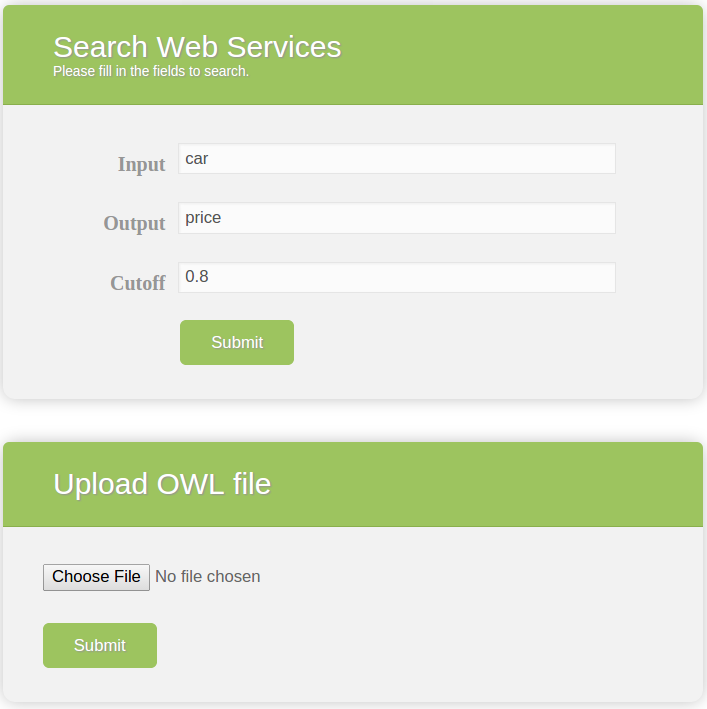
\includegraphics[width=\textwidth]{pics/search.png}
 \caption{\textbf{Screen-shot of Search Page}}
 \label{fig: search}
\end{figure}


\subsection{Indexing Web Services}
For indexation purpose, we define 7 categories (or dimensions) of Web Services as discussed in the preceding chapters. Each Input or Output vector is represented in this 7-dimension vector space. We assign a list of keywords on each of the seven categories. For our prototype system, we have have done this manually. We have some assigned some common input keywords for each category and some common output keywords to each category. This has been illustrated in Table ~\ref{tab: sample_keyword_output} and ~\ref{tab: sample_keyword_input}.

\begin{table}[h]
	\begin{center}
		\caption{\textbf{Sample Input Keywords Used for each Categories}}
		\label{tab: sample_keyword_input}
		\begin{tabular}{| p{0.2\textwidth} | p{0.6\textwidth} |}
			\hline
			\multicolumn{1}{|c|}{} & \multicolumn{1}{c|}{} \\
			\multicolumn{1}{|c|}{\textbf{Category}} & \multicolumn{1}{c|}{\textbf{Sample Input Keywords}} \\
			\multicolumn{1}{|c|}{} & \multicolumn{1}{c|}{} \\
			\hline
			Communication & Address, Code, Record, ZIP, Linguistic, Map, Media, Source, Analog, Digital \\ \hline
			Economy &  Dollar, Euro, Expense, Credit, Liability, Retail, Profit, Sale\\ \hline
			Education & Academic, Book, Author, Research, ISBN, Science, Reader, Radius\\ \hline
			Food & Butter, Bread, Beverages, Apple, Biscuit, Meat, Lemon, Honey, Pea, Tea\\ \hline
			Medical & Medical, Doctor, Hospital, Drug, Bed, Care, Visit, Clinic, Center\\ \hline
			Travel & Car, Bicycle, Longitude, Activity, Hill, Beach, Hike, Hotel, Capital\\ \hline
			Weapon & Ballistic, Destruct, Device, Missile, Projectile, Weapon, State, Power\\ \hline
		\end{tabular}
	\end{center}
\end{table}

\begin{table}[h!]
	\begin{center}
		\caption{\textbf{Sample Output Keywords Used for each Categories}}
		\label{tab: sample_keyword_output}
		\begin{tabular}{| p{0.2\textwidth} | p{0.6\textwidth} |}
			\hline
			\multicolumn{1}{|c|}{} & \multicolumn{1}{c|}{} \\
			\multicolumn{1}{|c|}{\textbf{Category}} & \multicolumn{1}{c|}{\textbf{Sample Output Keywords}} \\
			\multicolumn{1}{|c|}{} & \multicolumn{1}{c|}{} \\
			\hline
			Communication & Address, Interval, East, Phone, Time, Zone, URL, Information, Motion, Post\\ \hline
			Economy &  Firm, Intentional, Tax, Duty, Cost, Price, Bank, Fund, Income, Country, Total, Sold\\ \hline
			Education & Density, Scholarship, Article, Item, Liquid, Edit, Internal, Journal, Software\\ \hline
			Food & Beer, Price, Grain, Whiskey, Diet, Cereal, Breakfast, Lunch, Taste, Dough, Cola, Flavor\\ \hline
			Medical & Physical, Cost, Doctor, Test, Quality, Occupation, Specialty, Type, Bed, Internal\\ \hline
			Travel & Direction, Distance, Latitude, Longitude, Code, City, Area, Land, Hotel, Driver\\ \hline
			Weapon & Arrow, Price, Ship, Battle, Projectile, Weapon, State, Power, Technology\\ \hline
		\end{tabular}
	\end{center}
\end{table}
\par
Following a step-wise process of what we have implemented for indexing web services :
\begin{enumerate}
 \item \textbf{Document Parsing} - We implemented a OWLS Document Parser using Python. It extracted the required elements i.e \textbf{$<<$profile:hasinput$>>$} and \\ \textbf{$<<$profile:hasoutput$>>$} from all the OWLS files in our repository using Beautiful Soup package.
   \item \textbf{Algorithm for Constructing Input Vector} - After extraction we do the following for \textbf{$<<$profile:hasinput$>>$} element of each repository
   \begin{lstlisting}[language = bash, style = mystyle]
Vi = [0, 0, 0 ,0, 0, 0, 0]
for concept in concept-list #concept list is the list of 7 concept
	for keyword in concept.input_keylist #list of keywords
		if keyword is substring of <<profile:hasinput>>
			Vi[concept.no] += 1\end{lstlisting}
	\item \textbf{Algorithm for Constructing Output Vector} - Similarly, we do the following for \textbf{$<<$profile:hasout$>>$} element of each repository
   \begin{lstlisting}[language = bash, style = mystyle]
Vo = [0, 0, 0 ,0, 0, 0, 0]
for concept in concept-list #concept list is the list of 7 concept
	for keyword in concept.output_keylist #list of keywords
		if keyword is substring of <<profile:hasoutput>>
			Vo[concept.no] += 1 \end{lstlisting}
	\item \textbf{Implementing Vector Construction} -  UNIX Shell Script was used for construction of vectors. Powerful UNIX commands like \textbf{grep} were handy and had low-overhead.
	\item \textbf{Iterating through Dataset} - We wrote a python script to iterate through all the OWLS files in our dataset and apply all the above steps. After that we save the indexed Web Services in a file using space separated format.
\end{enumerate}

\subsection{Querying using Cosine Similarity}
We obtain the desired service interface from the user. For the requested interface (input and output), we create a request vector $R_i$ and $R_{o}$ of concepts using the same vector construction algorithm described in the previous section. Cosine similarity is found between $R_{i}$, $S_{i}$ and $R_{o}$, $S_{o}$ using a simple Python script by iterating through all the vectors of concepts in our dataset. We filter the results above a certain threshold and store the result in a temporary file.  Threshold value can be set by the user. But, threshold value greater than 0.7 is recommended for the retrieval of relevant services. A default value of 0.8 is used.

\section{Results and Analysis}
The results that we obtain are very encouraging. We are able to obtain very relevant web services given an interface. We have obtained this results with a very small set of keywords in each field (average 40 each). As such, with a large set of keywords in each category we should be able obtain a much better results.

\subsection{Sample Result}
A sample result set is illustrated in Table ~\ref{tab: sample_result}.
\begin{table}[H]
	\begin{center}
		\caption{\textbf{Sample Result of some Queries}}
		\label{tab: sample_result}
		\begin{tabular}{|>{\centering}p{0.1\textwidth}|>{\centering}p{0.1\textwidth}|>{\centering}p{0.1\textwidth}|>{\centering\arraybackslash}p{0.6\textwidth}|}
		\hline
		Input & Output & Theta & Services and Similarity \\ \hline
		Car & Price & 0.95 & 3wheeledcar\_price\_service (1.0), car\_price\_service (1.0), citycity\_arrowfigure\_service (1.0), lenthu\_rentcar\_service (0.972) \\ \hline
		Missile & Range & 0.9 & missile\_lendingrange\_service(0.971), missile\_givingrange(0.933), ballistic\_range\_service(0.918) \\ \hline
		Location & Distance & 0.9 & sightseeing\_service(1.0), DistanceInMiles(0.908), calculate\_betwee\_Location(0.903), surfing\_service(0.901) \\ \hline
		Medical & Bed & 0.5 & hospital\_investigatingaddress\_service(0.789), medicalclinic\_service(0.670), SeePatientMedicalRecords\_service(0.640) \\ \hline
		\end{tabular}
	\end{center}
\end{table}
\par
A screen shot of the sample result is also added. See Figure ~\ref{fig: result_screen}.
\begin{figure}[H]
 \centering
 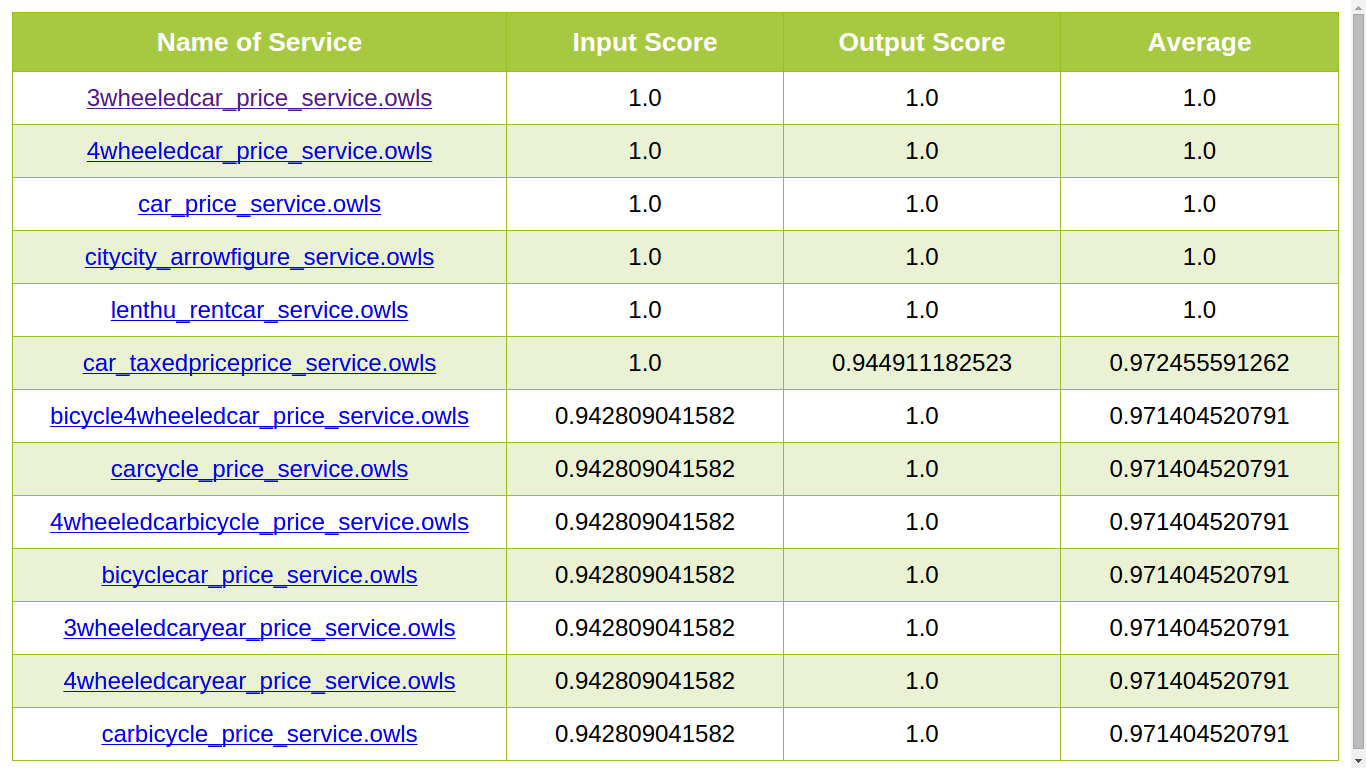
\includegraphics[width=\textwidth]{pics/results.png}
 \caption{\textbf{Screen-shot of Result Page}}
 \label{fig: result_screen}
\end{figure}


\subsection{Analysis}
The complexity analysis of the system for different events has been illustrated as follows:
\begin{itemize}
 \item \textbf{Indexing a single OWLS document} - The steps followed while indexing a single OWLS document and their complexity are:
 \begin{enumerate}
  \item Extract the input and output interface descriptions
  \item Compare the input keyword list and the output keyword list of all categories with the input and output interface description and create a vector from the comparison
 \end{enumerate}
 Step 1 is dependent on the length of the OWLS file and can be assumed to constant. Thus Step 1 takes constant time. \\ \par
 Let the number of keywords in each category, on an average be C. Since there are 7 categories, the number of keywords in the data set is $7C$. Our algorithm will compare each keyword in our data set with the input and output description. Thus the time taken will be proportional to $7C$. Thus Step 2 has $ \mathcal{O}(C)$ time complexity. \\ \par
 Thus the whole process of indexing a single OWLS document takes $\mathcal{O}(C)$ time.
 \item \textbf{Indexing the whole OWLS dataset} - To index the whole repository of web services we need to index each and every OWLS document by applying the algorithm mentioned before. Let the number of OWLS documents that the system has in it's repository be $N$. Since the algorithm to index a single OWLS document takes $\mathcal{O}(C)$ time (As shown in the previously), the algorithm to index the whole repository will take $\mathcal{O}(NC)$ time complexity.
 \item \textbf{Complexity of searching} - To search for a similar web service, the user will supply the input and the output he/she expects. Our algorithm will work in the following way :
 \begin{enumerate}
  \item Create a pair of vectors representing a pseudo OWLS file document the input and output supplied represents.
  \item Find the Cosine similarity of these vectors with the previously indexed values of all the OWLS documents in our repository and accept all those which are above a certain threshold value.
  \item Sort the result and display it to the user.
 \end{enumerate}
 Step 1 is equivalent to indexing a single OWLS document and hence takes $\mathcal{O}(C)$ time complexity. \\ \par
 Finding Cosine similarity between 2 OWLS documents takes constant time. In Step 2 we find the Cosine similarity of the pseudo OWLS document with each and every OWLS document. Let the number of OWLS documents in the system repository be N. Then Step 2 takes time of complexity $\mathcal{O}(N)$ \\ \par
 Step 3 is simple sorting that takes $\mathcal{O}(K\log{K})$ where K is the number of results after filtering using the given threshold. The maximum value of $K$ can be $N$. Thus the time taken by this step at most $\mathcal{O}(N\log{N})$. \\ \par
 Thus the complexity of searching for a similar web service is $\mathcal{O}(N) + \mathcal{O}(C) + \mathcal{O}(N\log{N})$.
\end{itemize}
Thus we can observe that the system is very efficient and scalable. It can easily handle large number of Web Services and still return result in a reasonable amount of time.

\section{Sample Code}
The python script to compute cosine similarity has been attached. See Figure ~\ref{fig: cosine} \\
A sample PHP code has also been attached which uploads a new Web Service Description File. See Figure ~\ref{fig: upload} \\
\begin{figure}[h]
 \centering
 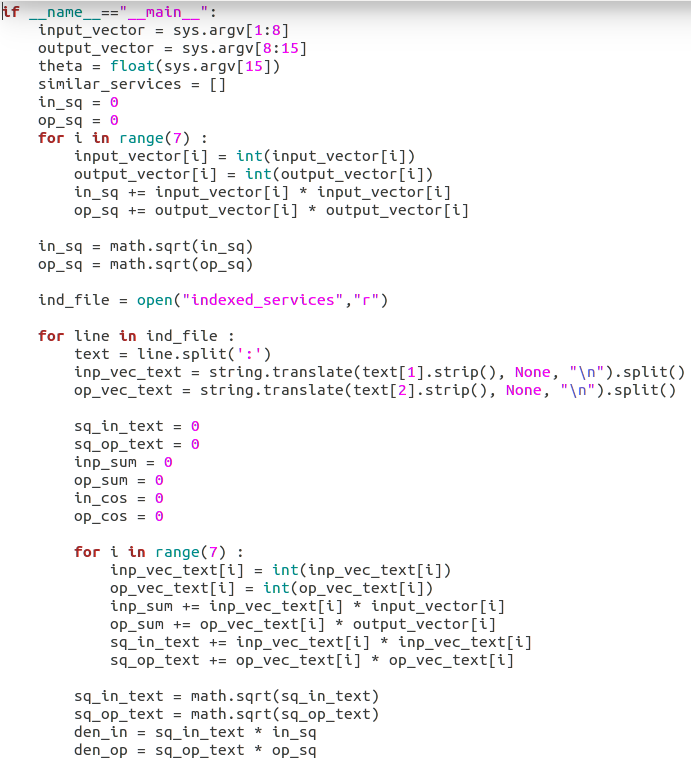
\includegraphics[width=\textwidth]{pics/cosine.png}
 \caption{\textbf{Python Script to Compute Cosine Similarity}}
 \label{fig: cosine}
\end{figure}

\begin{figure}[h]
 \centering
 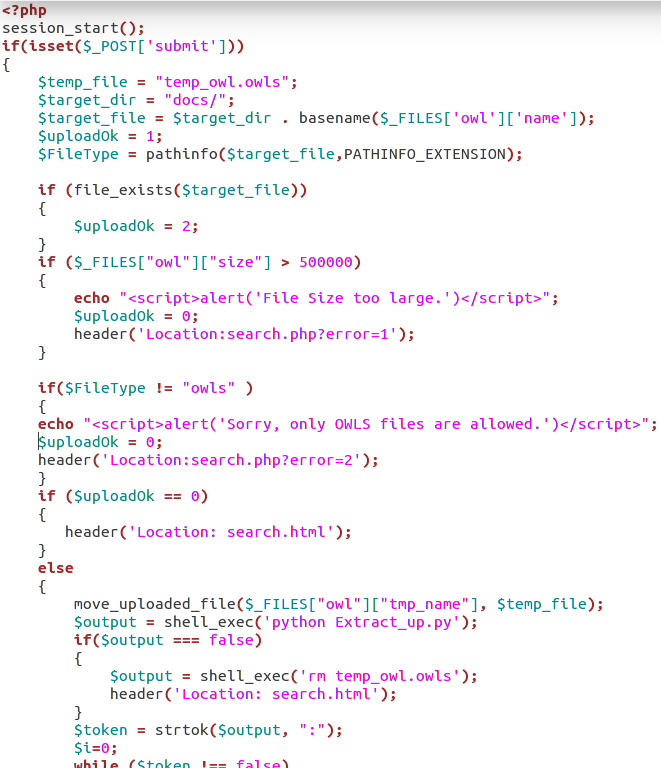
\includegraphics[width=\textwidth]{pics/upload.png}
 \caption{\textbf{PHP Script to Upload a new OWL-S File}}
 \label{fig: upload}
\end{figure}


\chapter{Conclusion and Future Work}
We have developed a basic search engine that uses only service interfaces. Our result looks promising. However, the current system still has a lot of scope for improvements which have been discussed in the following sections.
\section{Automatic Keyword Retrieval}
We manually indexed a set of keywords relevant to each category namely - economy, education, food, medical, travel, weapon and communication. However for a very large and diverse set of web services, it is not feasible to manually index appropriate keywords. One can make use of freely available repositories like WordNet to get the keywords related to a specific category. Moreover the keyword list should be dynamic i.e., the system should automatically learn new keywords and update the list. This can be achieved using machine learning techniques. A part of our problem can be modeled as a well known classification problem in the area of Machine Learning.
\section{Considering Other Parameters}
Currently our system constructs the appropriate vectors using only the words specified in the interface (input / output) of the web service. Better results could be obtained if we consider other parameters like functions and meta-data of a web services.

\pagebreak
\bibliographystyle{ieeetr}
\bibliography{biblio}
\addcontentsline{toc}{chapter}{Bibliography}
\addcontentsline{toc}{chapter}{Appendix Paper 1}
\includepdf[pages={1-9}]{paper1.pdf}
\addcontentsline{toc}{chapter}{Appendix Paper 2}
\includepdf[pages={1-6}]{paper2.pdf}
\end{document}